% ---------------------------------------------------------------------- %

\documentclass[letterpaper,10pt]{article}



\pagestyle{empty}

\usepackage[table]{xcolor}
\usepackage{color, colortbl}
\usepackage{tabularx}
\usepackage{amssymb}
\usepackage{enumerate}

\definecolor{LightGray}{gray}{0.9}

\usepackage{amsmath}
\usepackage{amscd}
\usepackage{url}

\usepackage{graphicx}


\title{Picking Travel Times}
\author{Seismo Group}
\date{\today}

\begin{document}
\maketitle

% ************************************************************* %
%                                                               %
%                       PICK TRAVEL TIMES                       %
%                                                               %
% ************************************************************* %

\section{Picking travel times}

In the terminal, cd into the directory with all the pkl files you want to run, and then do \verb"ttpick.py ___.bhz.pkl". You want to run either the \verb".bht" or \verb".bhz" files. 

A GUI should pop up if you successfully ran it.  

\begin{figure}[h!]
  \centering
  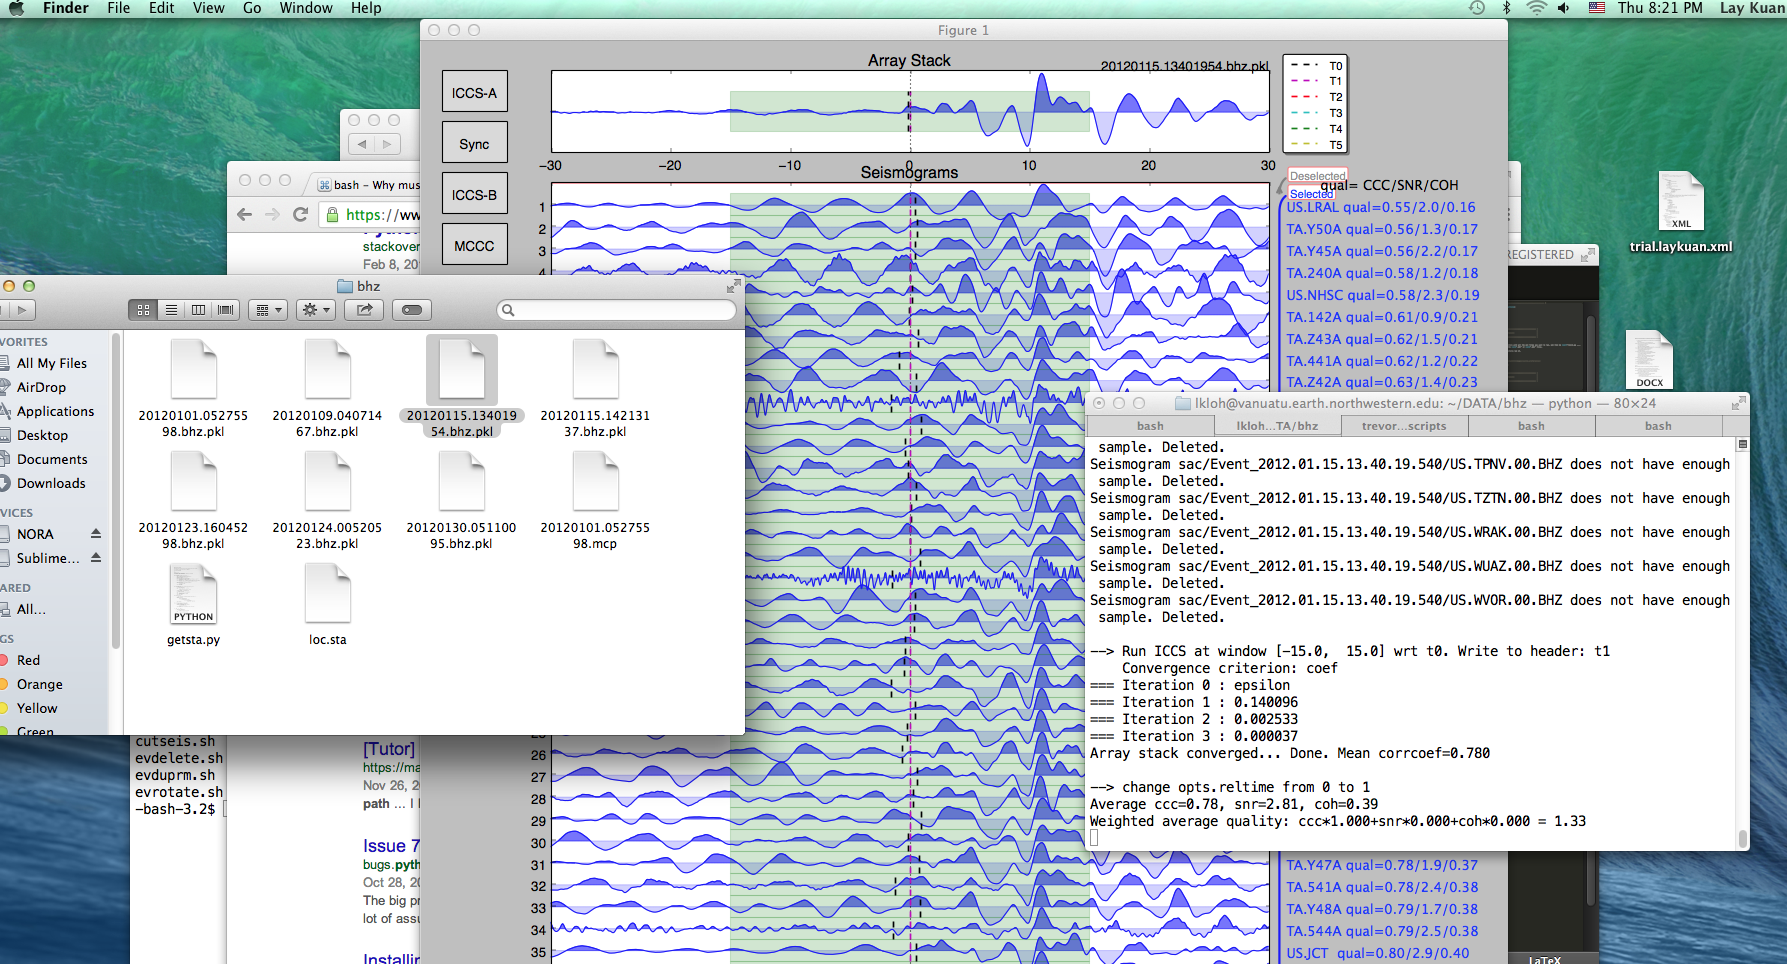
\includegraphics[width=0.5\textwidth]{images/pick_travel_times}
  \caption{Pick travel times}
  \label{fig:pick_travel_times}
\end{figure}

Remember to save your work periodically once you start picking your travel times, otherwise if AIMBAT crashes, you lose it. 

Hit \verb"MCCC", then \verb"SACP2". 

\section{Getting the stations of the seismograms kept}


% ************************************************************* %
%                                                               %
%                       PICK TRAVEL TIMES                       %
%                                                               %
% ************************************************************* %

\section{Getting the stations of the seismograms kept}


Run \verb"getsta.py" in the additional scripts (not on Github for now). It gives the unique list of stations where the seismograms came from. You need to run it with the list of all \verb"pkl" files chosen after you saved to. You so this \verb"./getsta.py *.pkl". 


\begin{figure}[h!]
  \centering
  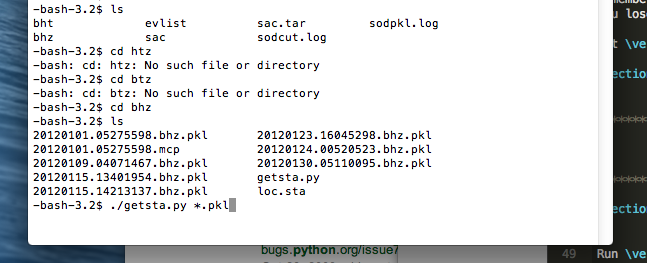
\includegraphics[width=0.5\textwidth]{images/count_stations}
  \caption{count stations}
  \label{fig:count_stations}
\end{figure}


\end{document}

% --------------------------------- END --------------------------------- %
